\documentclass[arhiv]{../izpit}
\usepackage{fouriernc}
\usepackage{xcolor}
\usepackage{fancyvrb}

\begin{document}

\izpit{Programiranje I: 1.~izpit}{19.\ januar 2023}{
  Čas reševanja je 120 minut.
  Veliko uspeha!
}

%%%%%%%%%%%%%%%%%%%%%%%%%%%%%%%%%%%%%%%%%%%%%%%%%%%%%%%%%%%%%%%%%%%%%%%

\naloga

\podnaloga
Napišite funkcijo \verb|permutacije : 'a -> 'a -> 'a -> ('a * 'a * 'a) list|, ki sprejme tri argumente in vrne seznam vseh možnih permutacij (elementi so med seboj različni), kjer vrstni red v seznamu ni važen.

\podnaloga
Napišite funkcijo \verb|zip_opt : 'a list -> 'b list -> ('a option * 'b option) list|, ki sprejme dva seznama in vrne seznam parov istoležnih elementov, ali vrednosti \verb|None|, če je kateri od seznamov krajši.

\begin{verbatim}
  # zip_opt [1; 2; 3] [true; false];;
  - : (int option * bool option) list =
  [(Some 1, Some true); (Some 2, Some false); (Some 3, None)]
\end{verbatim}
  
\podnaloga
Napišite funkcijo \verb|zip_default : 'a list -> 'b list -> 'a -> 'b -> ('a * 'b) list|, ki sprejme dva seznama in dve privzeti vrednosti ter vrne seznam parov istoležnih elementov. Če je kateri od seznamov krajši, naj funkcija uporabi ustrezno privzeto vrednost.

\podnaloga
Definirajmo tip \verb|response| kot:
\begin{verbatim}
  type response = Left | Middle | Right
\end{verbatim}
Napišite funkcijo
\begin{verbatim}
  distribute: ('a -> response) -> 'a list -> 'a list * 'a list * 'a list
\end{verbatim}
ki vrne tri sezname. V prvem so tisti elementi, kjer podana funkcija vrne \verb|Right|, v drugem tisti, kjer funkcija vrne \verb|Middle|, ostali pa v tretjem. Elementi v končnih seznamih naj nastopajo v enakem vrstnem redu, kot so nastopali v prvotnem seznamu.

\begin{verbatim}
# distribute (fun x -> if x < 0 then Left else if x = 0 then Middle else Right) 
    [1; 2; 3; 0; -1; 0; -2; 0; 4; 5; 6];;
- : int list * int list * int list =
([1; 2; 3; 4; 5; 6], [0; 0; 0], [-1; -2])
\end{verbatim}

\podnaloga
Vsoto $A + B$ lahko predstavimo s tipom
\begin{verbatim}
  type ('a, 'b) sum = Left of 'a | Right of 'b
\end{verbatim}
Definirajte preslikavi
\begin{verbatim}
  iso1 : (('a, 'b) sum -> 'c) -> ('a -> 'c) * ('b -> 'c)
  iso2 : ('a -> 'c) * ('b -> 'c) ->  (('a, 'b) sum -> 'c)
\end{verbatim}
ki ustrezata izomorfizmu $C^{A + B} \cong C^A \times C^B$.

%%%%%%%%%%%%%%%%%%%%%%%%%%%%%%%%%%%%%%%%%%%%%%%%%%%%%%%%%%%%%%%%%%%%%%%

\naloga

S tipom \verb|list_tree| predstavimo drevo, ki je sestavljeno bodisi iz listov z vrednostmi bodisi vozlišč, ki vsebujejo seznam poddreves tipa \verb|list_tree|.

\begin{verbatim}
  type 'a list_tree = Leaf of 'a | Node of 'a list_tree list
\end{verbatim}

\podnaloga
Napišite funkcijo \verb|map : ('a -> 'b) -> 'a list_tree -> 'b list_tree|, ki sprejme drevo in preslika elemente s podano funkcijo. 

\podnaloga
Napišite funkcijo \verb|count : 'a list_tree -> int|, ki sprejme drevo in vrne število listov v drevesu. Za vse točke mora biti funkcija repno rekurzivna.

\podnaloga
Napišite funkcijo \verb|apply : ('a -> 'b) list_tree -> 'a list_tree -> 'b list_tree|, ki sprejme dve drevesi in vrne novo drevo, kjer je vsak element rezultat aplikacije istoležne funkcije. Predpostavite lahko, da sta drevesi popolnoma enake oblike.

\podnaloga
Napišite funkcijo
\begin{verbatim}
  combine : ('a -> 'b) list_tree -> ('c -> 'a) list_tree -> ('c -> 'b) list_tree
\end{verbatim}
ki sprejme dve drevesi, katerih elementi so funkcije, in vrne novo drevo, kjer je vsak element kompozitum istoležnih funkcij. Predpostavite lahko, da sta drevesi popolnoma enake oblike. Za vsa (smiselna) drevesa mora veljati
\begin{verbatim}
  map (combine f g) t == (map f (map g t))
\end{verbatim}
vendar vam tega ni treba dokazovati.

\podnaloga
Napišite funkcijo
\begin{verbatim}
  apply_smart : ('a -> 'b) list_tree -> 'a list_tree ->
                ('a -> 'b) -> 'a -> 'b list_tree
\end{verbatim}
ki sprejme dve drevesi ter dve privzeti vrednosti (od katerih je prva funkcija) in vrne novo drevo, kjer je vsak element rezultat aplikacije funkcije iz prvega drevesa na istoležnem elementu iz drugega drevesa. Drevesi nista nujno enake oblike, ampak se lahko notranja vozlišča razlikujejo v številu otrok. Kjer število otrok ni enako, se vrsta otroka (list oz. vozlišče) v krajšem seznamu ujema s tistimi na začetku daljšega seznama. Namesto manjkajočih otrok (in njihovih potomcev) uporabite ustrezno privzeto vrednost, da dobite enako obliko kot jo ima drevo s presežkom otrok. Oblika končnega drevesa je unija oblik obeh vhodnih dreves.

\begin{verbatim}
# apply_smart ( Node [Node [Leaf (fun x -> x)]; Leaf (fun x -> x * 2)]) 
    (Node [Node []; Leaf 2; Leaf 4]) (fun x -> x * 110) 19
- : int list_tree = Node [Node [Leaf 19]; Leaf 4; Leaf 440]
\end{verbatim}

\[
  \mathtt{apply\_smart} \left(
  \vcenter{\hbox{\begin{tikzpicture}[level distance=0.9cm]
    \node {\texttt{N}}
      child {node {\texttt{N}}
        child {node {\texttt{L} $f_1$}}
      }
      child {node {\texttt{L} $f_2$}};
  \end{tikzpicture}}}
  ,\quad
  \vcenter{\hbox{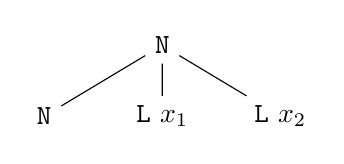
\begin{tikzpicture}[level distance=0.9cm]
    \node {\texttt{N}}
      child {node {\texttt{N}}}
      child {node {\texttt{L} $x_1$}}
      child {node {\texttt{L} $x_2$}};
  \end{tikzpicture}}}
  ,
  g
  ,
  y
  \right)
=
\vcenter{\hbox{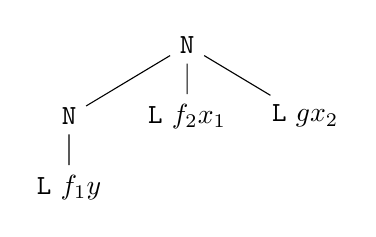
\begin{tikzpicture}[level distance=0.9cm]
  \node {\texttt{N}}
    child {node {\texttt{N}}
      child {node {\texttt{L} $f_1 y$}}
    }
    child {node {\texttt{L} $f_2 x_1$}}
    child {node {\texttt{L} $g x_2$}};
\end{tikzpicture}}}
\]

%%%%%%%%%%%%%%%%%%%%%%%%%%%%%%%%%%%%%%%%%%%%%%%%%%%%%%%%%%%%%%%%%%%%%%%

\naloga

\emph{Nalogo lahko rešujete v Pythonu ali OCamlu.}

Bacek Jon se nahaja pred gorskim grebenom, 
ki ga mora preplezati in se pri tem najesti
(trenutno še) živih zelišč, ki poraščajo 
gorovje, da mu bo na koncu ostalo čim več energije za nove potegavščine. Greben predstavimo z dvema seznamoma seznamov enakih dimenzij:
\begin{verbatim}
    60  50  40  30  20  30  40  50  60  70
  40  50  60  73  80      40  60  30  20  40
10  20  30  40  50          10  20  90  40  50
\end{verbatim}
oziroma v Pythonu kot
\begin{verbatim}
[                            [
  [60, 50, 40, 30, 20],        [30, 40, 50, 60, 70],
  [40, 50, 60, 73, 80],        [40, 60, 30, 20, 40],
  [10, 20, 30, 40, 50],        [10, 20, 90, 40, 50],
]                            ]
\end{verbatim}
v OCamlu pa podobno, samo s tipom \verb|array|.

Jon sprehod začne povsem spodaj levo na točki z 
vrednostjo 10 in konča povsem desno na točki 
z vrednostjo 50, pri tem pa se lahko premika 
zgolj po nepraznih sosednjih celicah (na posameznem 
kosu zemlje je vedno nenegativno število zelišč), 
kjer ga vodoravni premik stane 10 enot energije, 
navpični 12, diagonalni pa 14 enot energije.

Pozor: navpični premik pomeni, da bacek skoči na veljavno celico točno nad/pod trenutno, ki torej nikoli ni sosednja, za primer, to pomeni, da iz celice z vrednostjo 20 spodaj levo skoči naravnost gor na celico 60. 
V prvem delu se lahko bacek 
premika samo desno, navzgor, ali po pripadajoči 
diagonali desno navzgor, v drug polovici pa zgolj desno, navzdol
ali pa desno navzdol. 
Bacek ob premiku vsakič poje zelišča, ki so 
na lokaciji in s tem pridobi enako količino energije.

Vaša naloga je, da pripravite program, ki bo za dani greben
izračunal največjo količino energije, ki jo ima lahko bacek 
ob koncu poti in pripadajoče zaporedje premikov. Premike navzgor, navzdol, desno in diagonalno (neodvisno od smeri) označimo z \verb|U|, \verb|D|, \verb|R| in \verb|X|.
Predpostavite lahko, da bo čez greben vedno obstajala pot, pri kateri Jonu ne bo zmanjkalo energije.

Bacek lahko prikazan primer preskače tako, da mu na koncu ostane 533 enot energije, če sledi poti \verb|["R", "X", "R", "R", "R", "X", "R", "R", "R", "R", "D", "R", "R"]|.

\end{document}
